% Chapitre 12 -- ED-15 : le réseau triangulaire minimise-t-il l'énergie de point zéro harmonique ? (contre-exemple numérique)
% Sources : results/discovery_journal_2026/TOP20_final.json (pick 12), papers/prog_zero_point_optimality/{main.tex,AUDIT.md,REVISION.md,
% publication_meta.json,gen_numbers.tex,data/mechanism.json,data/rust_curv/}, results/programmes/2026-10-25/P2/GATE.md. Figure : code/fig12.py.
\chapter[Tester avant de prouver]{Tester avant de prouver : une idée naturelle qui ne tient pas}

\reference{Préprint du 25 octobre 2026, publié le 26 octobre 2026. doi:10.5281/zenodo.23653833}

\section*{L'idée en une image}

Des billes qui se repoussent, posées sur une table, s'arrangent en triangles, comme les
cellules d'une ruche. Pour une large famille de répulsions, ce rangement est le moins coûteux
quand les billes sont immobiles. Pour la répulsion
en cloche, c'est un résultat ancien de la littérature ; pour toute la famille, la preuve
publiée en 2026 a été produite par une IA et n'a pas encore été relue par des spécialistes.

Mais en physique quantique, rien n'est tout à fait immobile : même au zéro absolu, chaque
particule frissonne, et ce frisson coûte une énergie dite \og de point zéro\fg{}. L'idée
naturelle, notée QU-1 dans le projet, était que le champion au repos reste champion quand on
compte ce frisson. Elle a été écrite à l'avance, avec une estimation (six chances sur dix
qu'elle survive) et une règle : on ne chercherait à la démontrer que si elle passait d'abord
un test numérique. Elle ne l'a pas passé.

\begin{analogie}
Reliez les billes par des ressorts invisibles. Au repos, on compte la tension stockée dans les
ressorts : c'est là que le triangle gagne. Le frisson, lui, ressemble à une note que chaque
façon de vibrer fredonne sans arrêt ; l'énergie de point zéro est la somme de toutes ces
notes. Si l'on déforme un peu le rangement, certaines notes montent, d'autres descendent. Or
la hauteur d'une note varie comme la \emph{racine carrée} de la raideur : gains et pertes ne
se compensent plus comme pour la tension, et pour certaines cloches ce sont les notes graves
qui l'emportent.
\emph{Où l'image s'arrête :} il n'y a ni ressorts ni son ; une \og note\fg{} est une onde qui
parcourt tout le réseau, pas la vibration d'un ressort isolé, et le calcul compare des
arrangements figés, il ne suit aucun mouvement.
\end{analogie}

\section*{Ce qui a été fait}

Le test a porté sur douze répulsions de la famille : des cloches de cinq largeurs, deux
répulsions écrantées comme dans les plasmas, deux répulsions entre paires électron--trou de
matériaux en couches et trois puissances inverses de la distance. Pour plusieurs centaines de
formes de réseau, un programme calcule toutes les vibrations, écarte les réseaux instables (ceux où une
vibration s'emballe), puis additionne les notes.

Pour huit répulsions sur douze, on trouve un réseau stable, en losange légèrement aplati, qui
frissonne à moindre coût que le triangle. Pour la cloche $e^{-\pi r^2}$ : $1{,}4903$ contre
$1{,}5034$, un écart de $-0{,}0131$, environ dix mille fois l'erreur numérique estimée. Pour
les quatre autres, aucun meilleur réseau n'a été trouvé sur les points testés.

On a ensuite mesuré, pour la cloche $e^{-\pi a r^2}$ ($a$ grand : cloche étroite), la
\emph{courbure} $c$ de l'énergie de point zéro au triangle : positive, le triangle est au fond
d'un petit creux ; négative, il est sur un sommet. Sur 23 valeurs de $a$, $c$ est négative
pour $a$ entre $0{,}377$ et $1{,}581$ (figure). C'est cette surprise que le chapitre suivant
rend certaine, pour $a=1$ et le long d'un chemin précis.

\begin{encadre}
\textbf{À faire avec un crayon : la courbure prédit l'écart.} Pour un petit déplacement $d$
de la forme du réseau, l'écart d'énergie vaut environ $c\times d^2/0{,}75$ (le nombre
$0{,}75$ est un facteur géométrique fixe du triangle). Prenez $a=0{,}40$, où $c=-0{,}0799$,
et $d=0{,}02$ :
\[-0{,}0799\times0{,}0004/0{,}75\approx-0{,}0000426.\]
Un second programme du projet calcule directement les deux énergies, $1{,}3341042$ et
$1{,}3341470$ : l'écart vaut $-0{,}0000428$, presque la même chose. À $a=0{,}35$, où
$c=+0{,}0796$, la règle donne $+0{,}0000425$ et le calcul direct $+0{,}0000422$. Le signe
change entre $0{,}35$ et $0{,}40$ : c'est le bord gauche de la bande.
\end{encadre}

\section*{Comment on s'est assuré que ce n'est pas faux}

Le résultat principal est \niveau{X} \emph{une esquisse au crayon} : un calcul en virgule
flottante, qui guide sans prouver. Deux formules, programmées de quatre façons, donnent les
mêmes énergies. Un agent auditeur distinct en a écrit une cinquième, sans code commun : il
retrouve les deux énergies de la cloche $e^{-\pi r^2}$ à $10^{-12}$ près, la stabilité du
losange et le signe de $c$ à $a=1$ et $a=2$, mais n'a recalculé ni le reste de la bande, ni
les autres répulsions.

Les contrôles ont joué leur rôle. Le calcul des vibrations a été comparé à des différences
d'énergie obtenues en déplaçant vraiment les billes (33 cas, écart relatif au plus
$2\times10^{-7}$). Le réseau carré, qui doit sortir instable, sort instable. Pour la cloche
$a=2$, le même losange coûte \emph{plus} que le triangle : la méthode ne fabrique pas de
contre-exemple partout. Un premier \og meilleur\fg{} losange, à peine stable, a été
rétrogradé ouvertement.

\niveau{A} \emph{Le juge a regardé} pour 19 énoncés d'algèbre (des dérivées, et des lemmes sur
la rotation d'un tiers de tour, qui servent à montrer que la courbure est la même dans toutes
les directions) : le noyau de Lean,
le petit programme juge des preuves, les a vérifiés pas à pas, les axiomes restent dans la
liste courte autorisée, et un rejeu du module par le noyau est passé le 26 octobre. C'est ce
rejeu qui vaut à ce travail sa note de rigueur dans la sélection ; mais ces énoncés ne
certifient \emph{aucune} affirmation sur l'énergie. Quelques étapes intermédiaires sont
\niveau{C} \emph{un raisonnement, mené ici par des agents d'IA, que personne n'a vérifié à la
machine}, et trois résultats publiés sont \niveau{L}. Le verdict de l'auditeur,
\og accepter avec corrections\fg{}, demandait cinq corrections de texte, dont le
remplacement de \og fausse\fg{} par \og échoue numériquement\fg{} ; elles sont appliquées.
Aucun humain n'a relu ce travail.

\section*{Ce que ça ne dit pas}

\begin{limite}
\begin{itemize}
\item Ce n'est pas une preuve que l'idée est fausse : c'est un calcul, de niveau~X.
\item Au repos, le triangle reste le meilleur, et il reste stable ; seul le classement
  \og en frissonnant\fg{} change.
\item Vibrations traitées comme \og harmoniques\fg{}, réseaux réguliers à une bille par maille, deux
  dimensions ; les losanges sont imposés, pas des arrangements au repos.
\item Quatre répulsions ne sont pas prises en défaut sur un échantillon, qui n'est pas
  exhaustif. Pour une puissance inverse, le triangle est un creux local, et un losange plus
  lointain fait pourtant mieux de justesse : être battu et être sur un sommet sont deux choses
  différentes.
\item La bande vient de 23 points, étudiés après le test, sans préenregistrement ; rien n'est
  affirmé hors de $0{,}15\le a\le4$. La version restreinte de l'idée qui en découle n'est pas
  démontrée.
\item La force de Coulomb et celle des semi-conducteurs très minces sont exclues.
\end{itemize}
\end{limite}

C'est la leçon du chapitre : une idée plausible a été testée avant d'être prouvée, et c'est
l'échec du test, publié tel quel, qui a ouvert la piste suivante.

\section*{Pour aller plus loin}

Le papier (15 pages, en anglais) détaille les calculs, les contrôles et les énoncés Lean :
doi:10.5281/\allowbreak zenodo.23653833. Le même \og pas un minimum\fg{} a ensuite été établi
par un certificat (niveau~C d'ensemble : logique vérifiée par le juge, intégrales encadrées
hors du juge) pour la répulsion écrantée des plasmas : doi:10.5281/\allowbreak zenodo.23663551.

\begin{figure}[ht]
\centering
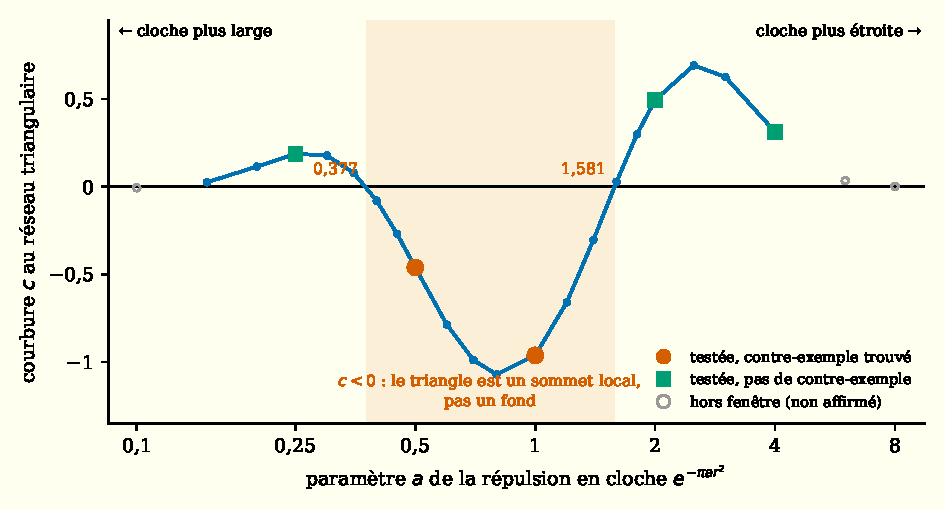
\includegraphics[width=\linewidth]{figures/c12_courbure_largeur}
\caption{Courbure de l'énergie de point zéro au triangle selon la largeur de la cloche : négative (zone ombrée) pour $0{,}377<a<1{,}581$ ; calcul en virgule flottante (niveau~X).}
\end{figure}
